%%%%%%%%%%%%%%%%%%%%%%%%%%%%%%%%%%%%%%%%%%%%%%%%%%%%%%%%%%%%%%%%%%%%%%%%%%
%%
%%   IPHIPI -- Agentic AI Mock Interview Platform
%%   Technical Presentation (LaTeX Beamer, 16:9)
%%
%%   Compile:  pdflatex PRESENTATION.tex   (twice for cross-refs)
%%   Output:   PRESENTATION.pdf (presentation-ready, full-screen via Acrobat)
%%
%%%%%%%%%%%%%%%%%%%%%%%%%%%%%%%%%%%%%%%%%%%%%%%%%%%%%%%%%%%%%%%%%%%%%%%%%%

\documentclass[aspectratio=169,10pt]{beamer}

\usepackage[utf8]{inputenc}
\usepackage[T1]{fontenc}
\usepackage{xcolor}
\usepackage{tikz}
\usepackage{amsmath,amssymb}
\usepackage{listings}
\usepackage{booktabs}
\usepackage{array}

\usetikzlibrary{arrows.meta,positioning,shapes,fit,calc,shadows.blur,backgrounds}

%%-------- IPHIPI brand palette --------%%
\definecolor{brand}{HTML}{5B67FF}
\definecolor{brandDark}{HTML}{2C3289}
\definecolor{brandLite}{HTML}{A8B8FF}
\definecolor{accent}{HTML}{8A6BFF}
\definecolor{ink}{HTML}{0A0D18}
\definecolor{paper}{HTML}{FBFBFE}
\definecolor{ruleline}{HTML}{D7D9E4}
\definecolor{codebg}{HTML}{F4F4F8}
\definecolor{ok}{HTML}{1F8A55}
\definecolor{warn}{HTML}{B5621A}
\definecolor{slidebg}{HTML}{080A14}
\definecolor{slidefg}{HTML}{E7EAF3}

%%-------- Beamer theme tweaks --------%%
\usetheme{default}
\useinnertheme{circles}
\setbeamertemplate{navigation symbols}{}

\setbeamercolor{background canvas}{bg=slidebg}
\setbeamercolor{normal text}{fg=slidefg}
\setbeamercolor{frametitle}{fg=white, bg=}
\setbeamercolor{title}{fg=white}
\setbeamercolor{subtitle}{fg=brandLite}
\setbeamercolor{structure}{fg=brand}
\setbeamercolor{item}{fg=brand}
\setbeamercolor{block title}{fg=white, bg=brand}
\setbeamercolor{block body}{bg=slidebg!85!white!4, fg=slidefg}
\setbeamercolor{alerted text}{fg=brandLite}

\setbeamerfont{frametitle}{size=\Large,series=\bfseries}
\setbeamerfont{title}{size=\Huge,series=\bfseries}

%%-------- frame title bar --------%%
\setbeamertemplate{frametitle}{
  \vspace{6pt}
  \begin{tikzpicture}[overlay,remember picture]
    \fill[brand] (current page.north west) rectangle ($(current page.north west)+(0.18,-0.5)$);
  \end{tikzpicture}\hspace{0.45cm}%
  \insertframetitle
  \par
  \vspace{-6pt}
  \textcolor{brand!50}{\rule{\dimexpr\linewidth-1cm}{0.4pt}}
}

%%-------- footline --------%%
\setbeamertemplate{footline}{
  \leavevmode%
  \hbox{%
    \begin{beamercolorbox}[wd=\paperwidth,ht=2.6ex,dp=1ex,leftskip=0.6cm,rightskip=0.6cm]{}
      \tiny\color{slidefg!55}
      IPHIPI \,\textbullet\, Agentic AI Mock Interview Platform
      \hfill
      \insertframenumber\,/\,\inserttotalframenumber
    \end{beamercolorbox}%
  }%
}

%%-------- listings --------%%
\lstdefinelanguage{json}{
  basicstyle=\ttfamily\scriptsize\color{slidefg},
  numbers=none,
  showstringspaces=false,
  breaklines=true,
  string=[s]{"}{"},
  morestring=[b]"
}
\lstset{
  backgroundcolor=\color{slidebg!90!white},
  basicstyle=\ttfamily\scriptsize\color{slidefg},
  frame=single,
  framerule=0pt,
  rulecolor=\color{brand!30},
  framesep=6pt,
  xleftmargin=4pt,
  xrightmargin=4pt,
  breaklines=true,
  showstringspaces=false,
  commentstyle=\color{slidefg!55},
  keywordstyle=\color{brandLite}\bfseries,
  stringstyle=\color{ok!80!white}
}

%%-------- TikZ helpers --------%%
\tikzset{
  block/.style={draw=brand!60, rounded corners=4pt, fill=brand!12, minimum width=3.0cm,
                minimum height=0.9cm, font=\sffamily\footnotesize\color{slidefg}, align=center,
                blur shadow={shadow blur steps=4}},
  store/.style={draw=accent!60, rounded corners=2pt, fill=accent!12, minimum width=2.6cm,
                minimum height=0.8cm, font=\sffamily\scriptsize\color{slidefg}, align=center},
  ext/.style={draw=ok!60, rounded corners=4pt, fill=ok!15, minimum width=2.7cm,
              minimum height=0.8cm, font=\sffamily\scriptsize\color{slidefg}, align=center},
  flow/.style={->,>={Stealth[length=2.2mm]}, semithick, draw=brandLite},
  sect/.style={draw=brandLite!30, dashed, rounded corners=6pt, inner sep=6pt},
  badge/.style={fill=brand, rounded corners=4pt, inner sep=4pt,
                font=\sffamily\bfseries\color{white}}
}

%%-------- a couple of slide helpers --------%%
\newcommand{\biglabel}[1]{\textcolor{brand}{\bfseries\large #1}}
\newcommand{\kpi}[2]{%
  \begin{tikzpicture}
    \node[draw=brand!60, fill=brand!10, rounded corners=8pt, minimum width=3.6cm, minimum height=1.6cm,
          align=center, font=\sffamily] {%
      \color{white}\bfseries\Large #1\\[2pt]
      \color{slidefg!75}\scriptsize #2%
    };
  \end{tikzpicture}}

\title{IPHIPI}
\subtitle{Agentic AI Mock Interview Platform}
\author{Technical Presentation}
\date{}

%%========================================================================%%
\begin{document}

%%========================== Title slide ==========================%%
\begin{frame}[plain]
  \begin{tikzpicture}[overlay,remember picture]
    \fill[brand]
      ($(current page.north west)+(0,-2.6)$)
      rectangle
      ($(current page.south west)+(0.3,0)$);
  \end{tikzpicture}
  \vspace{0.6cm}

  {\fontsize{52}{56}\selectfont\bfseries\color{white} IPHIPI}\\[0.3em]
  {\Large\color{brandLite} Agentic AI Mock Interview Platform}\\[2.4em]

  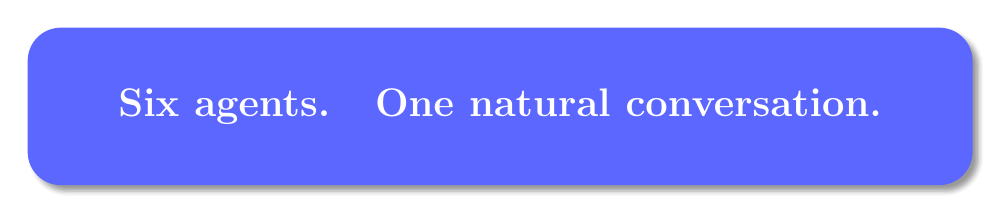
\begin{tikzpicture}
    \node[fill=brand,rounded corners=12pt,minimum width=12cm,minimum height=2.0cm,blur shadow]
      (logo) {};
    \node[white,font=\Large\bfseries] at (logo.center)
      {Six agents.\quad One natural conversation.};
  \end{tikzpicture}

  \vspace{1.6cm}
  \scriptsize\color{slidefg!75}
  \begin{tabular}{rl}
    \textbf{\color{brandLite}Live demo}  & \href{https://iphpi-hackthon.vercel.app}{iphpi-hackthon.vercel.app} \\
    \textbf{\color{brandLite}Repository} & \href{https://github.com/roshan5619/Intelligent_Mock_Interview_Agent}{github.com/roshan5619/Intelligent\_Mock\_Interview\_Agent} \\
    \textbf{\color{brandLite}Stack}      & Next.js \textbullet\ Groq Llama 3.3 70B \textbullet\ Gemini 2.0 \textbullet\ MediaPipe \\
  \end{tabular}
\end{frame}

%%========================== Problem ==========================%%
\begin{frame}{The problem we set out to solve}
  \vspace{0.2cm}
  \large Senior professionals (10--15+ years) cannot find rigorous,
  role-appropriate interview practice.\par
  \vspace{0.8cm}
  \footnotesize
  \begin{columns}[T,onlytextwidth]
    \column{0.32\textwidth}
      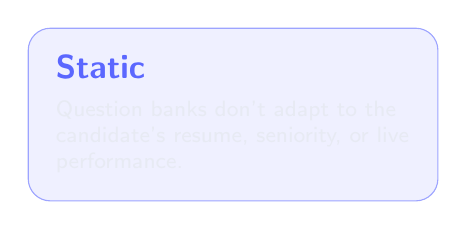
\begin{tikzpicture}
        \node[draw=brand!60,fill=brand!10,rounded corners=8pt,inner sep=10pt,
              text width=4.5cm,font=\sffamily\footnotesize\color{slidefg}]{
          \biglabel{Static} \\[4pt]
          Question banks don't adapt to the candidate's resume, seniority,
          or live performance.
        };
      \end{tikzpicture}
    \column{0.32\textwidth}
      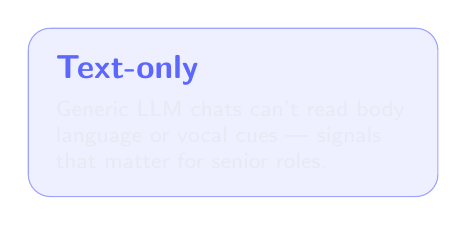
\begin{tikzpicture}
        \node[draw=brand!60,fill=brand!10,rounded corners=8pt,inner sep=10pt,
              text width=4.5cm,font=\sffamily\footnotesize\color{slidefg}]{
          \biglabel{Text-only} \\[4pt]
          Generic LLM chats can't read body language or vocal cues ---
          signals that matter for senior roles.
        };
      \end{tikzpicture}
    \column{0.32\textwidth}
      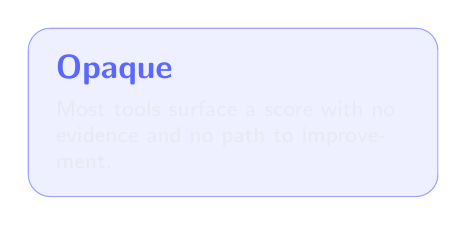
\begin{tikzpicture}
        \node[draw=brand!60,fill=brand!10,rounded corners=8pt,inner sep=10pt,
              text width=4.5cm,font=\sffamily\footnotesize\color{slidefg}]{
          \biglabel{Opaque} \\[4pt]
          Most tools surface a score with no evidence and no path to
          improvement.
        };
      \end{tikzpicture}
  \end{columns}
  \vspace{1.0cm}
  \color{brandLite}\bfseries\large
  IPHIPI is multimodal, adaptive, and explainable --- on free SOTA models.
\end{frame}

%%========================== Solution ==========================%%
\begin{frame}{What we built}
  \vspace{0.2cm}
  \begin{columns}[T,onlytextwidth]
    \column{0.55\textwidth}
      \large An \alert{agentic} platform that:
      \vspace{0.4em}
      \begin{itemize}\setlength\itemsep{0.7em}
        \item \textbf{Reads} the candidate's resume and infers the roles they
              can realistically land.
        \item \textbf{Conducts} a live multimodal interview (video + audio),
              dynamically generating questions and adapting difficulty.
        \item \textbf{Coaches} with per-dimension scores, evidence quotes,
              and concrete next steps.
      \end{itemize}
      \vspace{0.6em}
      \footnotesize\color{slidefg!75}
      Hands-free. Voice activity detection drives the conversation; no
      mic button to press.
    \column{0.45\textwidth}
      \vspace{0.3cm}
      \centering
      \begin{tabular}{c}
        \kpi{6}{specialized agents} \\[8pt]
        \kpi{4}{score dimensions} \\[8pt]
        \kpi{\$0}{infrastructure cost (free tiers)} \\
      \end{tabular}
  \end{columns}
\end{frame}

%%========================== User journey ==========================%%
\begin{frame}{End-to-end user journey}
  \vspace{0.2cm}
  \begin{tikzpicture}[
    node distance=2mm and 6mm,
    step/.style={draw=brand!60, rounded corners=4pt, fill=brand!10,
                 minimum width=2.3cm, minimum height=1.2cm,
                 font=\sffamily\scriptsize\color{slidefg}, align=center,
                 blur shadow={shadow blur steps=3}}
    ]
    \node[step] (s1) {Upload\\resume};
    \node[step, right=of s1] (s2) {Agent 1\\ context profile};
    \node[step, right=of s2] (s3) {JD-match\\ rank IPHIPI roles};
    \node[step, right=of s3] (s4) {Apply\\ see fit score};
    \node[step, right=of s4] (s5) {Mock\\ interview};
    \node[step, right=of s5] (s6) {Live\\ multimodal scoring};
    \node[step, right=of s6] (s7) {Coaching\\ report};

    \draw[flow] (s1)--(s2); \draw[flow] (s2)--(s3); \draw[flow] (s3)--(s4);
    \draw[flow] (s4)--(s5); \draw[flow] (s5)--(s6); \draw[flow] (s6)--(s7);
  \end{tikzpicture}

  \vspace{1.0cm}
  \footnotesize
  \begin{columns}[T,onlytextwidth]
    \column{0.5\textwidth}
      \biglabel{What the candidate sees}
      \begin{itemize}\setlength\itemsep{1pt}
        \item Animated fit score with matched skills + gaps
        \item Live transcript while they speak
        \item Real-time engagement / eye-contact / posture gauges
        \item Per-dimension report with evidence quotes
      \end{itemize}
    \column{0.5\textwidth}
      \biglabel{What runs behind the scenes}
      \begin{itemize}\setlength\itemsep{1pt}
        \item Six specialized agents, three in parallel per turn
        \item MediaPipe face + pose at 15 FPS in the browser
        \item Web Audio API for VAD + pitch + filler counting
        \item Groq Llama 3.3 70B for reasoning ($\sim$500 tok/s)
      \end{itemize}
  \end{columns}
\end{frame}

%%========================== Architecture diagram ==========================%%
\begin{frame}{High-level architecture}
  \vspace{-0.2cm}
  \centering
  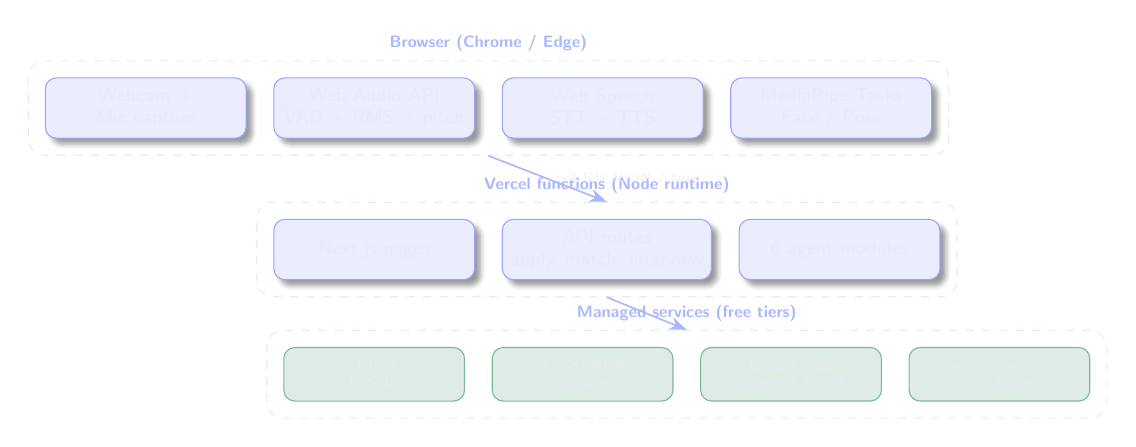
\begin{tikzpicture}[node distance=5mm and 4mm, scale=0.85, transform shape]

    %% Browser tier
    \node[block] (cam)   {Webcam +\\Mic capture};
    \node[block, right=of cam] (audio) {Web Audio API\\VAD + RMS + pitch};
    \node[block, right=of audio] (speech) {Web Speech\\STT + TTS};
    \node[block, right=of speech] (mp) {MediaPipe Tasks\\Face / Pose};
    \node[sect, fit=(cam)(audio)(speech)(mp),
          label={[font=\sffamily\scriptsize\bfseries\color{brandLite}]
          above:Browser (Chrome / Edge)}] (browser) {};

    %% Vercel tier
    \node[block, below=12mm of audio.south] (pages) {Next.js pages};
    \node[block, right=of pages] (api) {API routes\\apply, match, interview};
    \node[block, right=of api] (agents) {6 agent modules};
    \node[sect, fit=(pages)(api)(agents),
          label={[font=\sffamily\scriptsize\bfseries\color{brandLite}]
          above:Vercel functions (Node runtime)}] (vercel) {};

    %% External
    \node[ext, below=10mm of pages.south] (turso) {Turso\\libSQL};
    \node[ext, right=of turso] (blob) {Vercel Blob\\private};
    \node[ext, right=of blob] (groq) {Groq Cloud\\Llama 3.3 70B};
    \node[ext, right=of groq] (gemini) {Google Gemini\\2.0 Flash};
    \node[sect, fit=(turso)(blob)(groq)(gemini),
          label={[font=\sffamily\scriptsize\bfseries\color{brandLite}]
          above:Managed services (free tiers)}] (svc) {};

    \draw[flow] (browser.south) -- node[right,font=\tiny\color{slidefg!75}]
                                       {$\sim$2 KB JSON / turn} (vercel.north);
    \draw[flow] (vercel.south) -- (svc.north);
  \end{tikzpicture}

  \vspace{0.4cm}
  \footnotesize\color{slidefg!75}
  Raw video and raw audio never leave the browser --- only aggregated metric
  JSON ($\sim$2 KB per turn) reaches the server.
\end{frame}

%%========================== 6 Agents overview ==========================%%
\begin{frame}{The six agents}
  \vspace{0.2cm}
  \footnotesize
  \renewcommand{\arraystretch}{1.45}
  \begin{tabular}{@{}p{0.45cm}p{4.0cm}p{2.6cm}p{6.4cm}@{}}
    \toprule
    \color{brand}\textbf{\#} & \color{brand}\textbf{Agent} & \color{brand}\textbf{Runs in} & \color{brand}\textbf{Tech} \\
    \midrule
    1 & Context Understanding & Server          & Gemini 2.0 Flash (native PDF) + Groq fallback \\
    2 & Interview Orchestrator & Server         & Groq Llama 3.3 70B + adaptive heuristics \\
    3 & Audio Intelligence    & Browser$+$Server & Web Audio capture; Groq scoring \\
    4 & Visual Intelligence   & \alert{Browser only} & MediaPipe FaceLandmarker, PoseLandmarker, Blendshapes (\alert{pretrained CV, no LLM}) \\
    5 & Technical Evaluation  & Server          & Groq Llama 3.3 70B + rubric \\
    6 & Feedback \& Coaching  & Server          & Groq Llama 3.3 70B aggregating all per-turn signals \\
    \bottomrule
  \end{tabular}

  \vspace{0.8cm}
  \biglabel{Decoupling guarantees}\par\smallskip
  \footnotesize
  \begin{itemize}
    \item \textbf{One agent, one file.} Each agent is a pure typed function.
    \item \textbf{Prompts are data, not code.} System prompts live as \texttt{.md} files.
    \item \textbf{Storage is swappable.} Minimal interfaces; Turso $\rightarrow$ Postgres is a one-file change.
  \end{itemize}
\end{frame}

%%========================== Agent 1 ==========================%%
\begin{frame}{Agent 1 \textbullet\ Context Understanding}
  \vspace{0.2cm}
  \begin{columns}[T,onlytextwidth]
    \column{0.5\textwidth}
      \biglabel{Input}\par
      \footnotesize Resume PDF (or text).
      \vspace{0.6em}

      \biglabel{Pipeline}\par
      \footnotesize
      \begin{enumerate}\setlength\itemsep{1pt}
        \item Gemini 2.0 Flash reads the PDF natively (no \texttt{pdf-parse}).
        \item LLM emits a structured \texttt{ContextProfile}.
        \item \texttt{zod} validates the JSON shape; throws \texttt{ContextParseError} on drift.
        \item Fallback: \texttt{pdf-parse} $\rightarrow$ Groq when Gemini is rate-limited.
      \end{enumerate}

      \vspace{0.6em}
      \biglabel{Hard rule}\par
      \footnotesize Never invent skills the candidate doesn't claim.
    \column{0.5\textwidth}
      \biglabel{Output (excerpt)}
\begin{lstlisting}[language=json]
{
  "skills": ["Java", "Kafka", "..."],
  "years_total": 15,
  "roles": [...],
  "projects": [...],
  "seniority_signals":
     ["led team of 6", "..."],
  "inferred_roles": [{
    "role": "Backend",
    "confidence": 0.88,
    "rationale": "...",
    "matched_evidence": [...]
  }]
}
\end{lstlisting}
  \end{columns}
\end{frame}

%%========================== Agent 2 ==========================%%
\begin{frame}{Agent 2 \textbullet\ Interview Orchestrator}
  \vspace{0.1cm}
  \footnotesize
  Decides every next interviewer turn from the profile, agenda, transcript,
  multimodal metrics, and time budget.

  \vspace{0.4em}
  \begin{columns}[T,onlytextwidth]
    \column{0.55\textwidth}
      \biglabel{LLM output schema}
\begin{lstlisting}[language=json]
{
  "intent":  "probe_deeper" | "drop_difficulty"
           | "ramp_difficulty" | "clarify"
           | "encourage" | "wrap_up" | ...,
  "target_focus_area": string,
  "difficulty": 1..5,
  "question_style": "scenario" | "system_design"
                  | "behavioral_star" | ...,
  "next_question": string  // <=  50 words
}
\end{lstlisting}
    \column{0.45\textwidth}
      \biglabel{Adaptive difficulty (code, not prompt)}\par\smallskip
      \footnotesize
      We don't trust the LLM alone. Three deterministic heuristics layer
      on top of its decision:
      \vspace{4pt}
      \begin{itemize}\setlength\itemsep{2pt}
        \item 2 consecutive turns with confidence $<0.4$ $\rightarrow$ force \alert{drop\_difficulty} + prepend warm encouragement.
        \item 2 consecutive turns with correctness $>0.85$ $\rightarrow$ force \alert{ramp\_difficulty}.
        \item Time budget $<2$~min $\rightarrow$ force \alert{wrap\_up}.
      \end{itemize}
      \vspace{4pt}
      \tiny\color{slidefg!70}
      The LLM still writes the sentence; the policy is code.
  \end{columns}
\end{frame}

%%========================== Agent 3 ==========================%%
\begin{frame}{Agent 3 \textbullet\ Audio Intelligence}
  \vspace{0.2cm}
  \begin{columns}[T,onlytextwidth]
    \column{0.5\textwidth}
      \biglabel{Browser-side signals (50 ms samples)}\par\smallskip
      \footnotesize
      \begin{itemize}\setlength\itemsep{1pt}
        \item RMS mean + variance (volume envelope)
        \item Pitch $F_0$ + variance via autocorrelation
        \item Pause ratio, silence percentage
        \item WPM from transcript
        \item Filler rate (um / uh / like / you know)
      \end{itemize}

      \vspace{0.6em}
      \biglabel{Voice activity detection}\par\smallskip
      \footnotesize
      \begin{itemize}\setlength\itemsep{1pt}
        \item Start: RMS $>0.030$ for $\geq 200$ ms.
        \item End: RMS $<0.030$ for $\geq 900$ ms $\rightarrow$ auto-submit.
      \end{itemize}

    \column{0.5\textwidth}
      \biglabel{Server scoring (Groq, JSON mode)}
\begin{lstlisting}[language=json]
{
  "confidence":      0..1,
  "clarity":         0..1,
  "evidence":        "real signal quote",
  "signals_summary": "1-sentence interpretation"
}
\end{lstlisting}

      \vspace{0.4em}
      \biglabel{Rubric anchors}\par\smallskip
      \footnotesize
      Confidence HIGH ($>$0.7) when WPM $\in[110,160]$, fillers $<2$/min,
      pitch variance healthy, silence $<0.2$.\\
      Confidence LOW ($<$0.4) when WPM is erratic OR fillers $>6$/min OR
      pitch flat OR silence $>0.4$.
  \end{columns}
\end{frame}

%%========================== Agent 4 ==========================%%
\begin{frame}{Agent 4 \textbullet\ Visual Intelligence}
  \vspace{0.2cm}
  \begin{columns}[T,onlytextwidth]
    \column{0.5\textwidth}
      \biglabel{Browser (MediaPipe Tasks, WASM)}\par\smallskip
      \footnotesize
      \begin{itemize}\setlength\itemsep{1pt}
        \item FaceLandmarker (478 points + 52 blendshapes)
        \item PoseLandmarker (33 keypoints)
        \item Runs at $\sim$15 FPS, on-device
        \item Live face-mesh dots overlay the webcam --- visible proof the model is running
      \end{itemize}

      \vspace{0.5em}
      \biglabel{Per-turn aggregated metrics}\par\smallskip
      \footnotesize
      Eye-contact ratio, head-pose stability, posture score, smile,
      brow-raise, jaw-tension, blink rate.
    \column{0.5\textwidth}
      \biglabel{Deterministic server scoring}\par\smallskip
      \footnotesize Per the brief: \emph{pretrained CV over LLMs}. The
      server applies fixed weighted formulas --- no model call.
      \vspace{4pt}
      \scriptsize
      \begin{align*}
        \mathrm{engagement} &= 0.5 \\
                            &+ 0.25\,(e - 0.5) \\
                            &+ 0.15\,(s + b) \\
                            &+ 0.10\,(h - 0.5) \\[4pt]
        \mathrm{stress}     &= 0.5\,j + 0.3\,(1 - e) \\
                            &+ 0.2\,(1 - h)
      \end{align*}
      \tiny\color{slidefg!75}
      $e$ = eye contact, $s$ = smile, $b$ = brow raise, $h$ = head-pose
      stability, $j$ = jaw tension.
  \end{columns}
\end{frame}

%%========================== Agent 5 ==========================%%
\begin{frame}{Agent 5 \textbullet\ Technical Evaluation}
  \vspace{0.2cm}
  \footnotesize
  Scores each candidate answer against the question that triggered it.
  Calibration: most senior answers fall in 0.5--0.8; $\geq 0.9$ reserved
  for outstanding answers.

  \vspace{0.6em}
  \begin{columns}[T,onlytextwidth]
    \column{0.55\textwidth}
\begin{lstlisting}[language=json]
{
  "correctness":      0..1,
  "depth":            0..1,
  "specificity":      0..1,
  "concept_coverage": 0..1,
  "evidence_quote":   "MUST be a substring of the answer",
  "flags": [
    "hallucination" | "contradiction_with_resume"
                    | "off_topic" | "insufficient_detail"
  ]
}
\end{lstlisting}
    \column{0.45\textwidth}
      \biglabel{Why four dimensions, not one?}\par\smallskip
      \footnotesize
      A candidate can be \alert{correct but shallow}, or \alert{wide but
      inaccurate}. Splitting the score surfaces each failure mode in the
      final report.

      \vspace{0.6em}
      \biglabel{Why the evidence quote?}\par\smallskip
      \footnotesize
      Every per-turn rating must cite a substring of the actual answer.
      If we can't quote, we can't trust the score.
  \end{columns}
\end{frame}

%%========================== Agent 6 ==========================%%
\begin{frame}{Agent 6 \textbullet\ Feedback \& Coaching}
  \vspace{0.2cm}
  \footnotesize
  Runs \emph{once} at end of session. Aggregates every per-turn signal +
  the full transcript into a structured report.

  \vspace{0.6em}
  \begin{columns}[T,onlytextwidth]
    \column{0.55\textwidth}
      \biglabel{Output sections}\par\smallskip
      \footnotesize
      \begin{itemize}\setlength\itemsep{1pt}
        \item Headline summary (2 sentences)
        \item Per-dimension scores (technical, communication, confidence, engagement) 0--100
        \item Strengths (markdown bullets with evidence quotes)
        \item Improvements (markdown bullets with SPECIFIC, actionable steps)
        \item Behavioural insights (1--2 paragraphs interpreting audio + visual together)
        \item Next steps (3--5 concrete actions this week)
      \end{itemize}
    \column{0.45\textwidth}
      \biglabel{Final \emph{overall} weighting}\par\smallskip
      \footnotesize
      \[
        \mathrm{overall} = 0.35\,\tau + 0.30\,\kappa + 0.20\,\gamma + 0.15\,\eta
      \]
      where $\tau, \kappa, \gamma, \eta$ are technical, communication,
      confidence, engagement.

      \vspace{0.6em}
      \biglabel{The trick}\par\smallskip
      \footnotesize
      \texttt{overall} is \alert{recomputed server-side} after the LLM
      returns, so the model can't drift on the weighting.
  \end{columns}
\end{frame}

%%========================== Per-turn flow ==========================%%
\begin{frame}{What happens in one interview turn}
  \vspace{-0.2cm}
  \footnotesize
  \begin{tikzpicture}[
    node distance=2.5mm and 8mm, scale=0.9, transform shape,
    step/.style={draw=brandLite!40, rounded corners=3pt, fill=slidebg!85!white!4,
                 font=\sffamily\scriptsize\color{slidefg},
                 minimum width=3.0cm, minimum height=0.7cm, align=center},
    para/.style={draw=brand!60, fill=brand!15, rounded corners=3pt,
                 font=\sffamily\scriptsize\bfseries\color{white},
                 minimum width=2.8cm, minimum height=0.7cm, align=center}
    ]
    \node[step] (s1) {Browser flushes metrics};
    \node[step, below=of s1] (s2) {POST \texttt{/api/interview/turn}};
    \node[step, below=of s2] (s3) {Persist candidate turn};

    \node[para, right=18mm of s3] (a3) {Agent 3 (audio LLM)};
    \node[para, below=1mm of a3] (a4) {Agent 4 (CV math)};
    \node[para, below=1mm of a4] (a5) {Agent 5 (tech LLM)};

    \node[step, below=8mm of s3] (s4) {Persist all evaluations};
    \node[step, below=of s4] (s5) {Build 2-turn trends};
    \node[step, below=of s5] (s6) {Agent 2 decides next turn\\\emph{heuristics may override}};
    \node[step, below=of s6] (s7) {Return JSON $+$ TTS};

    \draw[flow] (s1)--(s2); \draw[flow] (s2)--(s3);
    \draw[flow] (s3.east) -| ([xshift=-3mm]a3.west) -- (a3.west);
    \draw[flow] (s3.east) -| ([xshift=-3mm]a4.west) -- (a4.west);
    \draw[flow] (s3.east) -| ([xshift=-3mm]a5.west) -- (a5.west);
    \draw[flow] (a3.south west) ..controls +(-0.8,-0.3) and +(0.8,0.3).. (s4.east);
    \draw[flow] (a4.south west) ..controls +(-0.8,-0.3) and +(0.8,0.3).. (s4.east);
    \draw[flow] (a5.south west) ..controls +(-0.8,-0.3) and +(0.8,0.3).. (s4.east);
    \draw[flow] (s4)--(s5); \draw[flow] (s5)--(s6); \draw[flow] (s6)--(s7);

    \node[font=\sffamily\scriptsize\color{brandLite}\bfseries,
          right=6mm of a3, anchor=west] {parallel};
  \end{tikzpicture}

  \vspace{0.4cm}
  \begin{block}{Latency math}
    \footnotesize
    $T_{\text{turn}} \approx \max(T_3, T_4, T_5) + T_2 \;\approx\;
    \text{1.0--1.5\,s parallel} + \text{1.0--1.5\,s orchestrator} \;\approx\;
    \mathbf{2\text{--}3\,s}$ total.
    Sequential execution would be $\sim$5--6 s. Parallel is the
    difference between conversational and awkward.
  \end{block}
\end{frame}

%%========================== JD-match scoring ==========================%%
\begin{frame}{Scoring \textbullet\ JD match}
  \vspace{0.2cm}
  \footnotesize
  Hybrid score in $[0, 100]$ for one (profile, job) pair:
  \[
    \mathrm{score}(P, J) = (0.4\,s_{\text{emb}} + 0.4\,s_{\text{skill}} + 0.2\,s_{\text{senior}}) \cdot 100
  \]

  \vspace{0.4em}
  \begin{columns}[T,onlytextwidth]
    \column{0.33\textwidth}
      \biglabel{Semantic}\par\smallskip
      \footnotesize Cosine similarity of Gemini 768-dim embeddings of
      profile-text and JD-text:
      \[
        s_{\text{emb}} = \mathrm{clamp}\!\left(\frac{\mathbf{e}_P \cdot \mathbf{e}_J}{\lVert \mathbf{e}_P\rVert\,\lVert\mathbf{e}_J\rVert}, 0, 1\right)
      \]
    \column{0.33\textwidth}
      \biglabel{Skill overlap}\par\smallskip
      \footnotesize Weighted by must-have ($w{=}1.0$) vs nice-to-have ($w{=}0.4$):
      \[
        s_{\text{skill}} = \frac{\sum_r w_r\,\mathbb{1}[r \in P]}{\sum_r w_r}
      \]
    \column{0.33\textwidth}
      \biglabel{Seniority fit}\par\smallskip
      \footnotesize Years-in-range step function: 1.0 in window, 0.7
      slightly out, 0.4 further out, 0.1 otherwise.
  \end{columns}

  \vspace{0.8em}
  \biglabel{Rationale}\par\smallskip
  \footnotesize
  After the deterministic score, the LLM writes a 2--3 sentence
  ``why this fits'' explanation \emph{grounded in the matched / gap
  lists}, never overriding the number.
\end{frame}

%%========================== Tech stack ==========================%%
\begin{frame}{The tech stack and why each piece}
  \vspace{0.2cm}
  \footnotesize
  \renewcommand{\arraystretch}{1.4}
  \begin{tabular}{@{}p{3.0cm}p{4.0cm}p{6.8cm}@{}}
    \toprule
    \color{brand}\textbf{Layer} & \color{brand}\textbf{Choice} & \color{brand}\textbf{Reason} \\
    \midrule
    Framework         & Next.js 15 (App Router) on Vercel & One repo, one deploy, one CDN. Server actions co-located with pages. \\
    Reasoning LLM     & Groq \alert{Llama 3.3 70B Versatile} & $\sim$500 tok/s; near-frontier reasoning; free 30 RPM / 14.4 K RPD. \\
    PDF + embeddings  & Google Gemini 2.0 Flash + \texttt{gemini-embedding-001} & Native PDF understanding; free embeddings. \\
    Vision (CV)       & MediaPipe Tasks (FaceLandmarker, PoseLandmarker, Blendshapes) & Pretrained, WASM, free, on-device. \\
    Voice             & Web Speech API (STT + TTS) + Web Audio API & Browser-native, zero infra, zero cost. \\
    Database          & Turso (libSQL) --- falls back to local SQLite & SQLite-compatible managed DB; same DAL works in Postgres v2. \\
    File storage      & Vercel Blob (private) & 1 GB free; signed download URLs via \texttt{head()}. \\
    Auth (prototype)  & HMAC-SHA256 signed cookie & No signup friction; magic-link in v2. \\
    \bottomrule
  \end{tabular}

  \vspace{0.6em}
  \biglabel{Multi-provider router}\par\smallskip
  \footnotesize
  Every LLM call goes through one typed entry point with auto-fallback
  $\text{Groq} \rightarrow \text{Gemini} \rightarrow \text{Ollama}$ on
  rate-limit or outage. The demo never hard-fails on one provider.
\end{frame}

%%========================== Design decisions ==========================%%
\begin{frame}{Key design decisions}
  \vspace{0.2cm}
  \footnotesize
  \begin{columns}[T,onlytextwidth]
    \column{0.5\textwidth}
      \biglabel{1. Browser does all multimodal capture + ML}\par\smallskip
      Privacy provable from the network tab. No GPU functions required.
      Per-turn payload is $\sim$2 KB, not megabytes of video.

      \vspace{0.7em}
      \biglabel{2. Single base model, six system prompts}\par\smallskip
      One latency profile, one cost profile, one failure mode. We tune
      \texttt{temperature} per agent, not the model.

      \vspace{0.7em}
      \biglabel{3. Async non-blocking evaluators}\par\smallskip
      Agents 3, 4, 5 run in parallel via \texttt{Promise.all}. Cuts
      candidate-perceived latency from $\sim$6 s to $\sim$2.5 s.

    \column{0.5\textwidth}
      \biglabel{4. Adaptive difficulty as code}\par\smallskip
      Hard heuristics override the LLM's intent on confidence dips,
      correctness streaks, or time pressure. Reliable, not hopeful.

      \vspace{0.7em}
      \biglabel{5. Pretrained CV over LLMs for body language}\par\smallskip
      MediaPipe gives us exact landmark coordinates at 15 FPS. A vision
      LLM would be 1000$\times$ slower and non-deterministic.

      \vspace{0.7em}
      \biglabel{6. Every score ships with evidence}\par\smallskip
      Every per-turn rating quotes a substring. Every report bullet
      cites a moment. ``You scored 71'' becomes ``You scored 71 because
      in turn 4 you led with the technology stack rather than the
      constraint it solved.''
  \end{columns}
\end{frame}

%%========================== Hands-free UX ==========================%%
\begin{frame}{The interview feels like a conversation}
  \vspace{0.2cm}
  \footnotesize
  Voice activity detection drives the loop. No mic button. No Send
  button.

  \vspace{0.8em}
  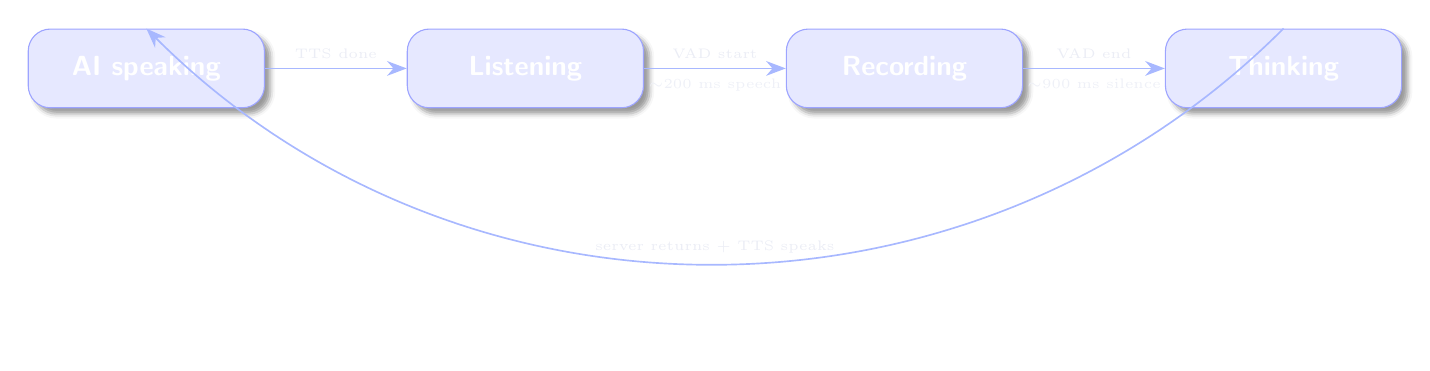
\begin{tikzpicture}[
    state/.style={draw=brand!60, rounded corners=8pt, fill=brand!15,
                  font=\sffamily\bfseries\color{white},
                  minimum width=3.0cm, minimum height=1.0cm, align=center,
                  blur shadow={shadow blur steps=3}},
    flow/.style={->,>={Stealth[length=2.5mm]}, semithick, draw=brandLite}
    ]
    \node[state] (a) {AI speaking};
    \node[state, right=18mm of a] (b) {Listening};
    \node[state, right=18mm of b] (c) {Recording};
    \node[state, right=18mm of c] (d) {Thinking};

    \draw[flow] (a) -- node[above,font=\tiny\color{slidefg!85}]{TTS done} (b);
    \draw[flow] (b) -- node[above,font=\tiny\color{slidefg!85}]{VAD start}
                       node[below,font=\tiny\color{slidefg!70}]{$\sim$200 ms speech} (c);
    \draw[flow] (c) -- node[above,font=\tiny\color{slidefg!85}]{VAD end}
                       node[below,font=\tiny\color{slidefg!70}]{$\sim$900 ms silence} (d);
    \draw[flow,bend left=45] (d.north) to node[above,font=\tiny\color{slidefg!85}]
                                            {server returns + TTS speaks} (a.north);
  \end{tikzpicture}

  \vspace{0.8em}
  \biglabel{Visible proof the agents are working}\par\smallskip
  \footnotesize
  Live face-mesh overlay on the webcam (478 dots) --- the candidate
  literally sees the vision model tracking their face. Live
  audio-waveform bar across the bottom of the cam. Eye-contact,
  engagement, posture gauges update every 250 ms.
\end{frame}

%%========================== Privacy ==========================%%
\begin{frame}{Privacy and security}
  \vspace{0.2cm}
  \footnotesize
  \begin{columns}[T,onlytextwidth]
    \column{0.5\textwidth}
      \biglabel{What never leaves the browser}\par\smallskip
      \begin{itemize}\setlength\itemsep{2pt}
        \item Raw video frames
        \item Raw audio buffers
        \item Microphone PCM data
      \end{itemize}
      \footnotesize
      Only the per-turn aggregated metric JSONs ($\sim$2 KB each) reach
      the server. The ``Local only'' badge in the cam corner reinforces
      this to the user.

      \vspace{0.8em}
      \biglabel{Resume protection}\par\smallskip
      \footnotesize
      Vercel Blob with \texttt{access:'private'}. The blob URL is
      internal-only; the server reads bytes back via \texttt{head()}
      with a token that signs the download URL.

    \column{0.5\textwidth}
      \biglabel{Cookie identity (prototype)}\par\smallskip
      \footnotesize
      \[
        \text{cookie} = \mathrm{b64url}(\text{payload})\,.\,\mathrm{b64url}\bigl(\mathrm{HMAC}_{K}(\text{payload})\bigr)
      \]
      Verification uses \texttt{timingSafeEqual}. Forgery requires
      \texttt{HMAC\_SECRET}.

      \vspace{0.6em}
      \biglabel{Ownership checks}\par\smallskip
      \footnotesize
      Every protected route asserts that the cookie's candidate ID matches the
      application / session being acted on. 401 / 404 otherwise.

      \vspace{0.6em}
      \biglabel{Rate-limit handling}\par\smallskip
      \footnotesize
      Provider router auto-falls-back Groq $\rightarrow$ Gemini $\rightarrow$ Ollama.
      User-facing banner only on full outage.
  \end{columns}
\end{frame}

%%========================== Limitations ==========================%%
\begin{frame}{Limitations we ship with}
  \vspace{0.2cm}
  \footnotesize
  \begin{itemize}\setlength\itemsep{4pt}
    \item \textbf{Browser support.} Web Speech + MediaPipe both need a
          Chromium-based browser. Firefox lacks \texttt{SpeechRecognition}.
          ``Type instead'' toggle is the universal fallback.
    \item \textbf{Concurrency.} Groq free tier is 30 RPM. Sustained
          concurrent interviews would saturate it; production needs a
          paid tier or a queue.
    \item \textbf{Resume formats.} PDF only. \texttt{.docx} and \texttt{.txt}
          deferred to v2.
    \item \textbf{Single language.} Prompts + STT default to English.
          Multilingual is a swap-in.
    \item \textbf{No real-time interruption.} The candidate must finish
          their turn before the next interviewer turn fires. Full duplex
          would require WebRTC.
    \item \textbf{Eye contact is from head pose}, not iris gaze. Sufficient
          for ``is the candidate facing the camera'' but cannot
          distinguish looking-at-notes from looking-at-AI.
    \item \textbf{VAD sensitivity.} A noisy environment may false-trigger.
          User can switch to text mode at any time.
  \end{itemize}
\end{frame}

%%========================== v2 roadmap ==========================%%
\begin{frame}{Next steps \textbullet\ v2 roadmap}
  \vspace{0.2cm}
  \footnotesize
  \begin{columns}[T,onlytextwidth]
    \column{0.5\textwidth}
      \biglabel{Near-term}
      \begin{itemize}\setlength\itemsep{2pt}
        \item Supabase magic-link auth + returning-candidate dashboard with interview history
        \item Deepgram (STT) + ElevenLabs (TTS) for broadcast-quality cross-browser voice
        \item Anthropic Claude Sonnet as a third LLM provider, routed for the report
        \item Mobile-friendly interview workspace
      \end{itemize}
    \column{0.5\textwidth}
      \biglabel{Production-readiness}
      \begin{itemize}\setlength\itemsep{2pt}
        \item Eval harness with golden interviews + LLM-as-judge regression tests
        \item Agent-decision audit log for compliance
        \item Upstash Redis token-bucket rate limiting
        \item ATS push (Greenhouse / Lever / Workday)
        \item GDPR consent, 30-day retention, opt-out, DPA
        \item Real-time interruption over WebRTC
      \end{itemize}
  \end{columns}
\end{frame}

%%========================== Demo ==========================%%
\begin{frame}{Live demo}
  \vspace{1.2cm}
  \centering
  
\begin{tikzpicture}
    \node[fill=brand,rounded corners=14pt,minimum width=14cm,minimum height=3.0cm,blur shadow]
      (demo) {};
    \node[white,font=\Huge\bfseries] at ($(demo.center)+(0,0.4)$)
      {iphpi-hackthon.vercel.app};
    \node[brandLite,font=\Large] at ($(demo.center)+(0,-0.5)$)
      {\textbullet\, Chrome or Edge \textbullet\, Webcam + mic on \textbullet\,};
  \end{tikzpicture}
  \vspace{1.2cm}

  \footnotesize\color{slidefg!85}
  \begin{tabular}{rl}
    \textbf{\color{brandLite}1.}  & Upload a PDF resume on \texttt{/match-me} \\
    \textbf{\color{brandLite}2.}  & Wait $\sim$25 s for Agent 1 + JD-match across all 6 roles \\
    \textbf{\color{brandLite}3.}  & Pick top-ranked role $\rightarrow$ apply $\rightarrow$ start interview \\
    \textbf{\color{brandLite}4.}  & Grant camera + mic $\rightarrow$ answer 3--4 turns hands-free \\
    \textbf{\color{brandLite}5.}  & End $\rightarrow$ get the per-dimension report with evidence quotes \\
  \end{tabular}
\end{frame}

%%========================== Q&A ==========================%%
\begin{frame}[plain]
  \begin{tikzpicture}[overlay,remember picture]
    \fill[brand]
      ($(current page.north west)+(0,-2.6)$)
      rectangle
      ($(current page.south west)+(0.3,0)$);
  \end{tikzpicture}
  \vspace{1.2cm}

  {\fontsize{60}{64}\selectfont\bfseries\color{white} Thank you.}\\[0.8em]
  {\LARGE\color{brandLite} Questions?}

  \vspace{3.2cm}
  \footnotesize\color{slidefg!75}
  \begin{tabular}{rl}
    \textbf{\color{brandLite}Live demo}  & \href{https://iphpi-hackthon.vercel.app}{iphpi-hackthon.vercel.app} \\
    \textbf{\color{brandLite}Repository} & \href{https://github.com/roshan5619/Intelligent_Mock_Interview_Agent}{github.com/roshan5619/Intelligent\_Mock\_Interview\_Agent} \\
    \textbf{\color{brandLite}Architecture doc} & \texttt{docs/ARCHITECTURE.tex} \\
    \textbf{\color{brandLite}Q\&A walkthrough} & \texttt{docs/INTERVIEW\_QA.html} \\
  \end{tabular}
\end{frame}

\end{document}
